\input{preamble}

\title{Computing architectures Part 1}
\institute{NTNU, IMF}
\date{January 19. 2018}
%\author{Aurélien Larcher}
\maketitle

%------------------------------------------------------------------------------
\section{Data representation}

%----------------------------------------
\begin{frame}
  \frametitle{Data representation}

Data is stored in binary in the memory:
\begin{itemize}
\item A \textit{bit} or binary digit is a value $0$ or $1$.
\item The basic unit is the \textit{byte} consisting of 8 bits,
\item Memory is as a contiguous array of bits 
\item These bits can be accessed by taking the address of the entry.
\item Memory may be addressed with a multiple of \textit{bytes},
\item Memory alignment denotes addressing the memory modulo $N$ bytes.
\end{itemize}

\bigskip
\scalebox{0.8}{
\begin{tabular}{c|cccc|cccc|c}
\hline
$\cdots$ & $\begin{bmatrix}\texttt{0x0A}\end{bmatrix}$ 
         & $\begin{bmatrix}\texttt{0x0B}\end{bmatrix}$ 
         & $\begin{bmatrix}\texttt{0x0C}\end{bmatrix}$ 
         & $\begin{bmatrix}\texttt{0x0D}\end{bmatrix}$
         & $\begin{bmatrix}\texttt{0x01}\end{bmatrix}$
         & $\begin{bmatrix}\texttt{0x02}\end{bmatrix}$ 
         & $\begin{bmatrix}\texttt{0x03}\end{bmatrix}$ 
         & $\begin{bmatrix}\texttt{0x04}\end{bmatrix}$ & $\cdots$ \\
\hline
\end{tabular}
}

\bigskip
Memory addressing: \textit{byte-addressed}, the lowest unit accessible is usually the \textit{byte}.
\end{frame}

%----------------------------------------
\begin{frame}
  \frametitle{Data representation}


A byte is a sequence of 8 binary digits.

\texttt{char} is encoded on a byte, it is the smallest integral type.
\begin{equation*}
\begin{bmatrix}b_7\;b_6\;b_5\;b_4\;b_3\;b_2\;b_1\;b_0 \end{bmatrix}
\end{equation*}

\begin{eqnarray*}
0 :&\qquad\begin{bmatrix}0\;0\;0\;0\;0\;0\;0\;0 \end{bmatrix}\\
1 :&\qquad\begin{bmatrix}0\;0\;0\;0\;0\;0\;0\;1 \end{bmatrix}\\
2 :&\qquad\begin{bmatrix}0\;0\;0\;0\;0\;0\;1\;0 \end{bmatrix}\\
3 :&\qquad\begin{bmatrix}0\;0\;0\;0\;0\;0\;1\;1 \end{bmatrix}\\
4 :&\qquad\begin{bmatrix}0\;0\;0\;0\;0\;1\;0\;0 \end{bmatrix}\\
\cdots&\qquad\cdots\\
255:&\qquad\begin{bmatrix}1\;1\;1\;1\;1\;1\;1\;1 \end{bmatrix}\\
\end{eqnarray*}

Conversion from binary to decimal representation of a number:
\begin{equation*}
\begin{bmatrix}b_k\;b_{k-1}\;\dots\dots b_1\;b_0 \end{bmatrix}_2 = \sum^{k}_{i = 0} b_i\;2^i
\end{equation*}

\end{frame}

%----------------------------------------
\begin{frame}
  \frametitle{Types: integral types}
ANSI/ISO C must support four signed and four unsigned data types:
\begin{enumerate}
\item \texttt{char}
\item \texttt{short}
\item \texttt{int}
\item \texttt{long}
\end{enumerate}

\medskip
ANSI requirements:
\begin{enumerate}
\item \texttt{short} and \texttt{int} are at least 16-bit long.
\item \texttt{long} is at least wider than \texttt{int} and not less than 32-bits.
\end{enumerate}

\end{frame}

%----------------------------------------
\begin{frame}
  \frametitle{Types: integer}

\begin{itemize}
\item Representation given number of binary digits: \textit{fixed width}
\item Signed integers, different strategies:
\begin{enumerate}
\item explicit sign: \textit{sign-magnitude}, \textit{one's complement}, \textit{two's complement}, \dots
\item implicit sign: \textit{excess-k}, \textit{base-2}, \dots
\end{enumerate}
\end{itemize}

\medskip
In explicit N-bit wide signed representations:
\begin{itemize}
\item S: sign bit
\item M: N-1 bits for the magnitude
\end{itemize}


  \begin{center}
    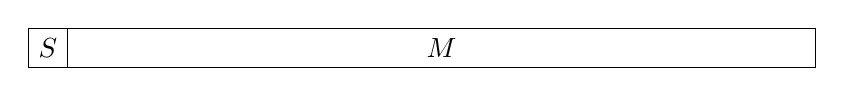
\begin{tikzpicture}[scale=0.5]
  \draw (0,0) rectangle (1,1);
  \draw (1,0) rectangle (20,1);
  \node at (0.5, 0.5) {$S$};
  \node at (10.5, 0.5) {$M$};
\end{tikzpicture}

  \end{center}

\end{frame}

%----------------------------------------
\begin{frame}
  \frametitle{Types: signed integers}
Two pieces of information need to be represented: the sign and the absolute value (or magnitude). 

\medskip
Different representations for the magnitude of negative numbers:
\begin{itemize}
\item \textit{sign-magnitude}: same as non-negative numbers
\begin{itemize}
\item zero is encoded in two ways
\item representation is natural thus not machine friendly
\end{itemize}
\item \textit{one's complement}: bitwise not of non-negative magnitude
\begin{itemize}
\item zero is encoded in two ways
\item \textit{end-around carry}: if 1 is carried it is added back (implementation difficulty)
\end{itemize}
\item \textit{two's complement}: bitwise not of non-negative magnitude + 1
\begin{itemize}
\item zero is encoded in only one way
\item can be seen as a circular encoding
\end{itemize}
\end{itemize}

\medskip
The \textit{two's complement} is the most widely used on modern architectures.

\end{frame}

%----------------------------------------
\begin{frame}
  \frametitle{Types: Sign-and-magnitude}
This representation is the intuitive way of expressing signedness: one signe bit and N-1 bit for the magnitude.


  \begin{center}
    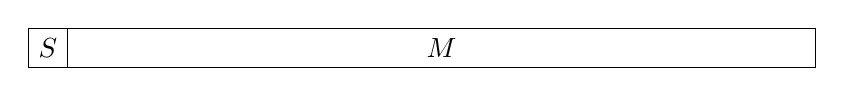
\begin{tikzpicture}[scale=0.5]
  \draw (0,0) rectangle (1,1);
  \draw (1,0) rectangle (20,1);
  \node at (0.5, 0.5) {$S$};
  \node at (10.5, 0.5) {$M$};
\end{tikzpicture}

  \end{center}

Range is $[-127, +127]$.
Zero is encoded as $-0$ and $+0$:
\begin{equation*}
\begin{bmatrix}0\;0\;0\;0\;0\;0\;0\;0 \end{bmatrix}
\end{equation*}
\begin{equation*}
\begin{bmatrix}1\;0\;0\;0\;0\;0\;0\;0 \end{bmatrix}
\end{equation*}

The definition of two zero and the impossibility of representing the subtraction in an efficient way are strong limitations.

\end{frame}

%----------------------------------------
\begin{frame}
  \frametitle{Types: One's complement}

\medskip
Negative values consists of applying a bitwise NOT operator to the unsigned representation.

\medskip
Range is $[-127, +127]$.

\medskip
Zero is encoded as $-0$ and $+0$:
\begin{equation*}
\begin{bmatrix}0\;0\;0\;0\;0\;0\;0\;0 \end{bmatrix}
\end{equation*}

\begin{equation*}
\begin{bmatrix}1\;1\;1\;1\;1\;1\;1\;1 \end{bmatrix}
\end{equation*}

\medskip
Hard to implement in pratice: \textit{end-around carry}: if $1$ is carried then it is added back. This representation has been abandoned.

\end{frame}

%----------------------------------------
\begin{frame}
  \frametitle{Types: Two's complement}

\medskip
Most used representation developed to workaround the double zero and the carry issue: if $1$ is carried is is simply ignored.

\medskip
Negative values consists of applying a bitwise \texttt{NOT} operator to the unsigned representation and adding $1$.

\medskip
Range is $[-128, +127]$:  notice that it is not symmetric anymore.

\medskip
Zero is encoded uniquely as:
\begin{equation*}
\begin{bmatrix}0\;0\;0\;0\;0\;0\;0\;0 \end{bmatrix}
\end{equation*}

\medskip
Representation of the bounds:

\begin{equation*}
+127:\qquad\begin{bmatrix}0\;1\;1\;1\;1\;1\;1\;1 \end{bmatrix}
\end{equation*}
\begin{equation*}
-127:\qquad\begin{bmatrix}1\;0\;0\;0\;0\;0\;0\;1 \end{bmatrix}
\end{equation*}
\begin{equation*}
-128:\qquad\begin{bmatrix}1\;0\;0\;0\;0\;0\;0\;0 \end{bmatrix}
\end{equation*}

\end{frame}

%----------------------------------------
\begin{frame}
  \frametitle{Types: Two's complement}

Motivation: the subtraction is consistent since:
\begin{equation*}
[+x]_2\;+\;[-x]_2 = [0]_2
\end{equation*}

\medskip
Take the simple example of: $+ 127 - 127$
\begin{equation*}
\begin{split}
+127\qquad\begin{bmatrix}0\;1\;1\;1\;1\;1\;1\;1 \end{bmatrix}\\
-127\qquad\begin{bmatrix}1\;0\;0\;0\;0\;0\;0\;1 \end{bmatrix}\\
\ = 0 \qquad 1 \begin{bmatrix}0\;0\;0\;0\;0\;0\;0\;0 \end{bmatrix}
\end{split}
\end{equation*}

\end{frame}

%----------------------------------------
\begin{frame}
  \frametitle{Real numbers}

\medskip
The difficulty to represent infinitely many real numbers with a finite number of bits: only some numbers can be represented exactly.

\medskip
A number is \textit{binary rational} if it can be written exactly in base $2$.

\medskip
Other number are then approximated: the error due to the representation is coined \textit{round-off error}.

\end{frame}


%----------------------------------------
\begin{frame}
  \frametitle{Real numbers}

\begin{multline*}
\begin{bmatrix}527.2\end{bmatrix}_{10} = 1\cdot 2^{+9} + 1\cdot 2^{+3} + 1\cdot 2^{+2} + 1\cdot 2^{1} + 1\cdot 2^{0}  \\+ 0\cdot 2^{-1} + 0\cdot 2^{-2} + 1\cdot 2^{-3}+ 1\cdot 2^{-4} + \cdots
\end{multline*}

\begin{multline*}
\begin{bmatrix}527.2\end{bmatrix}_{10} \approx \bigl(+1\bigr)\cdot 2^{+9}\;\bigl(1\cdot 2^{+0} + 1\cdot 2^{-6} + 1\cdot 2^{-7} + 1\cdot 2^{-8} \\
+ \cdot 2^{-9} + 0\cdot 2^{-10} + 1\cdot 2^{-11}+ 1\cdot 2^{-12}\bigr)
\end{multline*}

\begin{equation*}
\begin{bmatrix}527.2\end{bmatrix}_{10} \approx \bigl(+1\bigr)\cdot 2^{+9}\;\begin{bmatrix}1.0000011110011\end{bmatrix}_{2}
\end{equation*}

\begin{equation*}
\bigl(+1\bigr)\cdot 2^{+9}\;\begin{bmatrix}1.0000011110011\end{bmatrix}_{2} = 527.1875
\end{equation*}

\end{frame}

%----------------------------------------
\begin{frame}
  \frametitle{Fixed point numbers}
  \begin{itemize}
  \item How to encode decimal numbers in the binary system?
  \item First alternative:
   \begin{enumerate}
   \item Use $x$ bits to represent digits before the radix point (integer),
   \item and $y$ bits to represent digits after the radix points,
   \end{enumerate}
    where $x+y = w$ for a $w$ bit representation: fixed point representation.
  \item Problem: only a fixed range of numbers can be represented i.e.
    $2^x + 1 - 2^{-y}$ is the largest.
  \item Called fixed point since the point is fixed. The
    \emph{absolute} accuracy is constant.
  \end{itemize}


\begin{center}
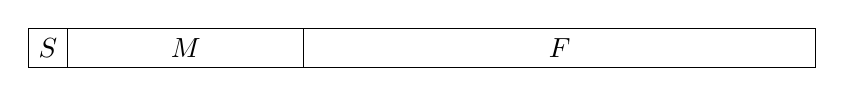
\begin{tikzpicture}[scale=0.5]
  \draw (0,0) rectangle (1,1);
  \draw (1,0) rectangle (7,1);
  \draw (7,0) rectangle (20,1);
  \node at (0.5, 0.5) {$S$};
  \node at (4, 0.5) {$M$};
  \node at (13.5, 0.5) {$F$};
\end{tikzpicture}
\end{center}

\end{frame}


%----------------------------------------
\begin{frame}
  \frametitle{Types: floating-point}

\begin{center}
Infinitely many real numbers $\rightarrow$ finite number of bits of representation
\end{center}

Representation and behaviour defined by the IEEE-754 standard:
\begin{itemize}
\item Definition of \textit{guard digits} to reduce error e.g when substracting nearby numbers.
\item Definition of algorithms for:
\begin{enumerate}
\item addition/substraction
\item multiplication/division
\item square root
\end{enumerate}
\end{itemize}

\medskip
\begin{itemize}
\item Constraints: implementations should produce the same results as algorithms
\item Goal: ensure portability across platform
\end{itemize}

\medskip
Bypassing IEEE-754 can be specified to the compiler: faster to the expense of accuracy.

\end{frame}

%----------------------------------------
\begin{frame}
  \frametitle{Floating point numbers}
  \begin{itemize}
  \item A better idea is to let the comma position ``float''.
  \item Floating-point numbers have constant \emph{relative} accuracy.
  \item Allows us to represent a much larger range of numbers.
  \end{itemize}
  \begin{center}
    \input{\figs/tma4280/float}
  \end{center}
  \begin{itemize}
    \item[S] The sign bit (1 bit).
    \item[E] The exponent
    \item[F] The significand (formerly: mantissa)
  \end{itemize}
\end{frame}

%----------------------------------------
\begin{frame}
  \frametitle{Floating point numbers}
  Thus;
  \[
    V = (-1)^S \cdot 2^{E-B}\cdot M
  \]
  where the significand $M$ is defined as
  \[
    M = \underbrace{1}_{\times2^0} .
    \overbrace{\underbrace{b_1}_{\times2^{-1}}
      \underbrace{b_2}_{\times2^{-2}}\ldots}^{F}
  \]
  for \textit{normalized} numbers (most common). Here $B$ is the \emph{bias}. Common
  precisions:
  \begin{center}
    \input{\data/precision}
  \end{center}

The \textit{fractional} part is stored as \textit{sign-magnitude} and the \textit{exponent} as \textit{biased representation}.

\end{frame}

%----------------------------------------
\begin{frame}
  \frametitle{Floating point numbers}
  \begin{itemize}
  \item The \emph{bias} allows us to give a bias to large or small numbers
    (large or small exponents).
  \item Since we use a finite representation, we have a finite precision.
  \item Smallest and largest numbers:
    \begin{align*}
      V_\text{min} &= 1\cdot 2^{1-127}\cdot 1 = 2^{-126} = 1.17\ldots 10^{-38} \\
      V_\text{max} &= 1\cdot 2^{254-127}\cdot 2 = 3.40\ldots 10^{38}.
    \end{align*}
  \item More important: The smallest \emph{relative} difference between numbers
    we can represent
    \[
      2^{-23} = 1.19....10^{-7}.
    \]
    i.e.~under perfect circumstances we have about 7 digits of accuracy.
  \item The \textit{denormalization} allows to represent smaller numbers.
  \end{itemize}
\end{frame}

%----------------------------------------
\begin{frame}
  \frametitle{Denormalization}

The smallest numbers can be represented using the first bit.

\medskip
Minimum: $2^{1-B-F}$

\medskip
Single precision: $2^{-149}\;\approx 1.6\cdot 10^{-45}$
Double precision: $2^{-1074}\;\approx 5.0\cdot 10^{-324}$
\end{frame}

%----------------------------------------
\begin{frame}
  \frametitle{Floating point operations}
  \begin{itemize}
    \item A very useful estimate for the size of a scientific code is the total
      number of floating point operations performed.
    \item Floating point operations: $+$, $-$, $\times$, $/$
    \item A floating point operation is called a FLOP.
    \item It is tempting to use \SI{}{\flop} for the plural, but that is \emph{not} the norm. Rather, \SI{}{\flop} is used about Floating-Point OPeration per Second, which is a very useful
      performance metric.
    \item $\SI{3}{\flop}$ or $\SI{1}{\flop}$
  \end{itemize}
\end{frame}

%----------------------------------------
\begin{frame}
  \frametitle{Floating point limitations}
  \begin{itemize}
  \item Finite precision of the number representation leads to accuracy issues: the \textit{condition} measure the error propagation for a given function.
  \item Subtraction: $1.2345\cdot 10^4$ minus $1.2344\cdot 10^4$.
    \begin{align*}
      & 1.2345 \cdot 10^4 - 1.2344 \cdot 10^4 \\
      &= (1.2345 - 1.2344) \cdot 10^4 \\
      &= \textcolor{red}{0.0001} \cdot 10^4 \\
      &= 1.0000 \cdot 10^0
    \end{align*}
    We have only a single digit of accuracy! This is called \emph{cancellation}, due to the \textit{truncation} error.
  \item Example where this matters: Approximations of derivatives
    \[
      \frac{\text{d}f}{\text{d}x} \approx \frac{1}{h}\left( f(x+h) - f(x) \right)
    \]
  \end{itemize}
\end{frame}

%----------------------------------------
\begin{frame}
  \frametitle{Floating point limitations}
  \begin{itemize}
  \item Addition: $1.2345\cdot 10^4$ plus $1.0000\cdot 10^0$.
    \begin{align*}
      & 1.2345 \cdot 10^4 + 1.0000 \cdot 10^0 \\
      &= (1.2345 + 0.0001) \cdot 10^4 \\
      &= 1.2346 \cdot 10^4
    \end{align*}
    OK!
  \item Addition: $1.2345\cdot 10^4$ plus $1.0000\cdot 10^{-1}$.
    \begin{align*}
      & 1.2345 \cdot 10^4 + 1.0000 \cdot 10^{-1} \\
      &= (1.2345 + 0.0000) \cdot 10^4 \\
      &= 1.2345 \cdot 10^4
    \end{align*}
    Adding the small number has no effect: the number of \textit{significant} digits is crucial.
  \end{itemize}
\end{frame}

%----------------------------------------
\begin{frame}
  \frametitle{Data models}
  \begin{center}
    \input{\data/data-models}
  \end{center}

\medskip

\begin{itemize}
\item Exotic platform may use alternate models (ILP64, SILP64).
\item Important for portability: avoid invalid assumption regarding conversion.
\end{itemize}

\end{frame}

%----------------------------------------
\begin{frame}
  \frametitle{Endianness}

Integral data types are stored packed by \textit{bytes}, 2 options.

The binary word can be stored with bytes from \textit{left-to-right} or from \textit{right-to-left}.

\bigskip
Big-Endian: Most-Significant Byte is first:

\bigskip
\begin{tabular}{c|cccc|c}
\hline
$\cdots$ & $\begin{bmatrix}\texttt{0x0A}\end{bmatrix}$ 
         & $\begin{bmatrix}\texttt{0x0B}\end{bmatrix}$ 
         & $\begin{bmatrix}\texttt{0x0C}\end{bmatrix}$ 
         & $\begin{bmatrix}\texttt{0x0D}\end{bmatrix}$ & $\cdots$ \\
\hline
\end{tabular}

\bigskip
Little-Endian: Least-Significant Byte is first:

\bigskip
\begin{tabular}{c|cccc|c}
\hline
$\cdots$ & $\begin{bmatrix}\texttt{0x0D}\end{bmatrix}$ 
         & $\begin{bmatrix}\texttt{0x0C}\end{bmatrix}$ 
         & $\begin{bmatrix}\texttt{0x0B}\end{bmatrix}$ 
         & $\begin{bmatrix}\texttt{0x0A}\end{bmatrix}$ & $\cdots$ \\
\hline
\end{tabular}

\medskip
This is especially important when dealing with IO formats.

\end{frame}

%------------------------------------------------------------------------------
\section{Single processor system}

%----------------------------------------
\begin{frame}
  \frametitle{Ideal single processor model}

In this part a processor is a conceptual unit able to load data, perform computations and store the result.

\medskip
The Von Neumann architecture:
  \begin{center}
    \scalebox{0.8}{
      \begin{tikzpicture}[
  block/.style={
    draw=darkblue,
    fill=cadet,
    shape=rectangle,
    rounded corners=1mm,
    text height=1.5ex,
    text depth=.25ex,
  },
  l1/.style={
    minimum height=8mm,
    minimum width=4cm,
  },
  ops/.style={
    minimum height=8mm,
    minimum width=4cm,
    align=right,
  },
  inst/.style={
    minimum height=28mm,
    minimum width=16mm,
  },
  line/.style={
    thick,
    draw=darkblue,
  }]
  \node[block, l1] (CPU) {Processor};
  \node[block, l1, fill=salmon, right=15mm of CPU] (MEM) {Memory};
  \draw[line, <->] (CPU.east) -- (MEM.west);
\end{tikzpicture}

    }
  \end{center}

\begin{itemize}
\item Processor and Memory are connected by a Bus.
\item Memory contains programs and data (i.e no Harvard which splits them).
\end{itemize}

\medskip
Real models deviate from this idealized model.\\[2ex]
$\rightarrow$ Detailed knowledge of the hardware is crucial.

\bigskip
Three basics types: \textit{processors}, \textit{memory}, \textit{connections}\\[2ex]
$\rightarrow$ Each categories has performance improvement techniques: pipelining, block caching, patterns.

\end{frame}

%----------------------------------------
\begin{frame}
  \frametitle{Single processor systems: RISC architecture}
  \begin{center}
    \scalebox{0.8}{
      \input{\figs/tma4280/single-proc}
    }
  \end{center}
\end{frame}

%----------------------------------------
\begin{frame}
  \frametitle{Single processor systems: memory hierarchy}
  \begin{center}
    \scalebox{0.8}{
      \input{\figs/tma4280/memory-hierarchy}
    }
  \end{center}
\end{frame}



%----------------------------------------
\begin{frame}
  \frametitle{Single processor systems: memory hierarchy}

  Typical memory access times for the MIPS R14000 processor. The numbers
  represent number of clock cycles.
  \begin{center}
    \input{\data/memory-times}
  \end{center}
\end{frame}

%----------------------------------------
\begin{frame}
  \frametitle{Single processor systems: memory hierarchy}

Locality is crucial to achieve performance, it is usually based on heuristics.

\begin{enumerate}
\item Temporal locality: how likely will we need the data in the future?
\item Spatial locality: how likely will we need the data in the block of memory?
\end{enumerate}

\medskip
Memory stall cycles: number of cycles during which the processor is stalled, waiting for a memory access.

\medskip
Caching is an improvement to the Von Neumann model: higher speed of smaller memory, keep some data in a fast memory if it is reused.
  
\end{frame}

%----------------------------------------
\begin{frame}
  \frametitle{Pitfalls}

The increasing gap between processor clock frequencies and the lower-level memory makes the processor \textit{starve} for instructions.

\medskip
Techniques were developed to circumvent this issue.
\end{frame}

%------------------------------------------------------------------------------
\section{Performance}


%----------------------------------------
\begin{frame}[fragile]
  \frametitle{Different types of parallelism}

\begin{enumerate}
\item Memory-Level Parallelism (MLP): several pending memory operations.
\vspace{2ex}
\item Instruction-Level Parallelism (ILP): how many instruction can be scheduled simultaneously. 
\vspace{2ex}
\item Data-Level Parallelism (DLP): execute one instruction on multiple data.
\vspace{2ex}
\item Thread-Level Parallelism (DLP): executing several threads of computation on the same processor.
\end{enumerate}

\medskip
The main notion to understand the bottlenecks is \textit{data dependencies}.

\end{frame}

%----------------------------------------
\begin{frame}[fragile]
  \frametitle{Performance factors}

At the single processor level, several techniques to takes advantage of \textit{Instruction-Level Parallelism} (ILP):
\begin{itemize}
\item instruction pipelining,
\item superscalar execution,
\item branch prediction,
\item speculative execution,
\item vectorization (SIMD),
\item prefetching.
\end{itemize}

\medskip
Vectorization using additional \textit{vector units} (SIMD) can exploit \textit{Data parallelism}.

\end{frame}


%----------------------------------------
\begin{frame}[fragile]
  \frametitle{Pipelining}

Multiple instructions are overlapped in execution: take advantage of parallelism existing between actions required to execute an instruction.

\medskip
View of an assembly line: different task performed by different operators.

\medskip
Prototypical Five-Stage RISC:
\begin{tabular}{c|l|l|}
\textbf{IF}  & Instruction-Fetch  & \\
\textbf{ID}  & Instruction-Decode & \\
\textbf{EX}  & Execute            & \\
\textbf{MEM} & Memory Access      & Load/Store \\
\textbf{WR}  & Write in Register  & Register-Register, ALU, Load\\
\end{tabular}

The theoretical speed-up for a $N$--stage is $N$, but:
\begin{itemize}
\item Overhead for controlling the pipeline.
\item Lowest common denominator: speed is limited to the slowest element.
\item Hazards: data dependencies, branch misprediction.
\end{itemize}

\end{frame}

%----------------------------------------
\begin{frame}[fragile]
  \frametitle{Pipelining/Vectorization}

Hockney formula: time to operate on vectors of size N
\begin{equation*}
t_N = (s + l + (N - 1)) \tau
\end{equation*}

\medskip
\begin{enumerate}
\item $s$: startup phase, time to prepare the pip and fetch operands
\item $l$: number of cycles to fill the pipe
\item $\tau$: time for one clock cycle
\end{enumerate}

\medskip
Operation rate: $r = n / t_n$ number of operations per unit time.

\end{frame}

%----------------------------------------
\begin{frame}[fragile]
  \frametitle{Pipelining/Vectorization}
  Consider the fused scalar multiplication and vector addition:
  \begin{align*}
    \bm c = \bm a + \gamma \bm b
  \end{align*}
  We can write this operation as the loop
  \begin{center}
    \begin{tabular}{c}
\begin{lstlisting}[style=fortran]
for i=1,n
  c(i) = a(i) + gamma * b(i)
end
\end{lstlisting}
    \end{tabular}
  \end{center}
  A single iteration is performed in a certain number of stages. These stages
  can be viewed as a pipeline.
\end{frame}

%----------------------------------------
\begin{frame}
  \frametitle{Superscalar operations}
  \begin{align*}
    \bm c = \bm a + \gamma \bm b
  \end{align*}

  \begin{center}
    \input{\figs/tma4280/superscalar} \\
    Fused multiply and add (FMADD)
  \end{center}
\end{frame}

%----------------------------------------
\begin{frame}
  \frametitle{Vectorization}
  Modern processors contain vector (SIMD, Single Instruction Multiple Data)
  units. This allows to apply the same operation to multiple data in parallel.
  In modern Intel (Sandy Bridge, Haswell) chips, the vector units are also
  superscalar (both AVX and SSE).

  Three ways to enable SIMD usage in your programs:
  \begin{itemize}
  \item autovectorizing compilers (ICC),
  \item hand-written assembly,
  \item intrinsics (built-in functions)
  \end{itemize}
\end{frame}


%----------------------------------------
\begin{frame}
  \frametitle{Caching techniques}
Memory latency is a bottleneck: use of memory hierarchy to take advantage of \textit{space locality} and \textit{time locality}.

\medskip
Scientific computing involving:
\begin{itemize}
\item long data streams,
\item very few conditionals,
\item regular memory access patterns
\end{itemize}
is suitable for performance improvement by caching.

  \begin{center}
    \input{\figs/tma4280/direct-mapped-cache}
  \end{center}
  \[
    \text{Memory address} =
    \underbrace{b_1 \ldots b_k}_{\text{tag bits}}
    \underbrace{b_{k+1} \ldots b_{N}}_{\text{cache address}}.
  \]
\end{frame}

%----------------------------------------
\begin{frame}
  \frametitle{Caching techniques}
Problem: the memory latency has increased relative to the CPU frequency, moving data from/to the memory is expensive relative to computational cost on the CPU.

\medskip
\begin{enumerate}
\item Cache hit: the processor find the data in the cache
\item Cache miss: the processor does not find the data in the cache
\end{enumerate}

\medskip
Cache miss penalty depends on:
\begin{enumerate}
\item the memory latency: time to access the first block.
\item the memory bandwidth: time of transfer per unit block.
\end{enumerate}

Using locality to buffer reuse of reoccurring items.
\end{frame}

%----------------------------------------
\begin{frame}
  \frametitle{Caching techniques}
\medskip
Different cache strategies based on different implementations of:
\begin{enumerate}
\item block placement: where is the cached data stored?
\item block identification: how is the data found in the cache?
\item block replacement: how to decide which block should be replaced?
\item write strategy: if data is changed, how to write to the main memory?
\end{enumerate}
\end{frame}

%----------------------------------------
\begin{frame}
  \frametitle{Caching techniques}

Block placement:
\begin{itemize}
\item \textit{direct-mapped}: block can be placed only at one location
\item \textit{fully associative}: block can be placed anywhere
\item \textit{set associative}: block can be placed in a restricted set of places, ``n-way associative'' means that nw
\end{itemize}

\medskip
Block identification: address tag to find the block. 


\end{frame}

%----------------------------------------
\begin{frame}
  \frametitle{Caching techniques}

Block replacement:
\begin{itemize}
\item \textit{Random}: block replaced is chosen randomly
\item \textit{FIFO}: First-In-First-Out
\item \textit{LRU}: Least-Recently-Used
\item \textit{pseudo-LRU}: Least-Recently-Used with heuristics
\end{itemize}

Write strategy:
\begin{itemize}
\item \textit{Write-though}: write to main memory directly
\item \textit{Write-back}: write a next synchronization
\end{itemize}
\end{frame}

%----------------------------------------
\begin{frame}
  \frametitle{Direct mapped cache}
  \begin{center}
    \input{\figs/tma4280/direct-mapped-cache}
  \end{center}
  \[
    \text{Memory address} =
    \underbrace{b_1 \ldots b_k}_{\text{tag bits}}
    \underbrace{b_{k+1} \ldots b_{N}}_{\text{cache address}}.
  \]
\end{frame}

%----------------------------------------
\begin{frame}[fragile]
  \frametitle{Direct mapped cache}
  \begin{center}
    \begin{tabular}{c}
\begin{lstlisting}[style=fortran]
for i=1,n
  c(i) = a(i) + b(i)
end
\end{lstlisting}
    \end{tabular}
  \end{center}

  If the vectors are precisely the same length as a cache line, we get cache
  trashing.

  \begin{center}
    \input{\figs/tma4280/cache-trashing}
  \end{center}
\end{frame}

\begin{frame}
  \frametitle{Adjacent memory layout}
  \begin{center}
    \input{\figs/tma4280/adjacent-memory} \\
    Interleaving the vectors in memory avoids cache trashing.
  \end{center}
\end{frame}

%----------------------------------------
\begin{frame}
  \frametitle{Other cache strategies}
  \begin{itemize}
  \item Fully associative cache: \emph{all} bits in a memory address are used as
    tag bits, none of them as cache address. All cache addresses are available.
  \item $n$-way associative cache: uses $m$ fewer bits for cache address than a
    direct mapped cache, thus freeing up a choice of $n = 2^m$ cache addresses
    for each chunk. This is a good compromise between direct mapped cache and
    fully associative cache
  \end{itemize}
\end{frame}

\begin{frame}
  \frametitle{Speculative and Out-of-Order execution}

During the execution there may exist dependencies between data such that the process needs to wait for data before proceeding further.

\medskip
\begin{enumerate}
\item \textit{in-order}: pause of execution until data is fetched
\item \textit{out-of-order}: instruction waits but execution of other instructions with non-dependent data is scheduled.
\end{enumerate}

\end{frame}

%----------------------------------------
\begin{frame}
  \frametitle{Conclusion}
  \begin{itemize}
  \item As the processor clock frequency increasing, memory latency became the bottleneck.
  \item Many techniques developed to increase concurrency of tasks: instruction parallelism and overlapping of data movement.
  \item Complexity of single-processors and technological reached a limit calling for other types of parallelism to achieve performance.
  \end{itemize}

Timeframe:
  \begin{itemize}
  \item 1986--2000: the gap between memory and CPU performance increases, development of memory hierarchies. 
  \item 2005: Intel cancels the $4$GHz Pentium 4, limits of ILP are reached (hear/power/complexity).
  \item 2005--Now: Development of multichip--multicore platforms:
\begin{enumerate}
\item NUMA: memory hierarchies improved to ensure coherence and consistency.
\item TLP: explosion of the thread model.
\end{enumerate}
  \end{itemize}

\end{frame}

\input{postamble}
